\documentclass[twoside]{book}

% Packages required by doxygen
\usepackage{fixltx2e}
\usepackage{calc}
\usepackage{doxygen}
\usepackage[export]{adjustbox} % also loads graphicx
\usepackage{graphicx}
\usepackage[utf8]{inputenc}
\usepackage{makeidx}
\usepackage{multicol}
\usepackage{multirow}
\PassOptionsToPackage{warn}{textcomp}
\usepackage{textcomp}
\usepackage[nointegrals]{wasysym}
\usepackage[table]{xcolor}

% Font selection
\usepackage[T1]{fontenc}
\usepackage[scaled=.90]{helvet}
\usepackage{courier}
\usepackage{amssymb}
\usepackage{sectsty}
\renewcommand{\familydefault}{\sfdefault}
\allsectionsfont{%
  \fontseries{bc}\selectfont%
  \color{darkgray}%
}
\renewcommand{\DoxyLabelFont}{%
  \fontseries{bc}\selectfont%
  \color{darkgray}%
}
\newcommand{\+}{\discretionary{\mbox{\scriptsize$\hookleftarrow$}}{}{}}

% Page & text layout
\usepackage{geometry}
\geometry{%
  a4paper,%
  top=2.5cm,%
  bottom=2.5cm,%
  left=2.5cm,%
  right=2.5cm%
}
\tolerance=750
\hfuzz=15pt
\hbadness=750
\setlength{\emergencystretch}{15pt}
\setlength{\parindent}{0cm}
\setlength{\parskip}{3ex plus 2ex minus 2ex}
\makeatletter
\renewcommand{\paragraph}{%
  \@startsection{paragraph}{4}{0ex}{-1.0ex}{1.0ex}{%
    \normalfont\normalsize\bfseries\SS@parafont%
  }%
}
\renewcommand{\subparagraph}{%
  \@startsection{subparagraph}{5}{0ex}{-1.0ex}{1.0ex}{%
    \normalfont\normalsize\bfseries\SS@subparafont%
  }%
}
\makeatother

% Headers & footers
\usepackage{fancyhdr}
\pagestyle{fancyplain}
\fancyhead[LE]{\fancyplain{}{\bfseries\thepage}}
\fancyhead[CE]{\fancyplain{}{}}
\fancyhead[RE]{\fancyplain{}{\bfseries\leftmark}}
\fancyhead[LO]{\fancyplain{}{\bfseries\rightmark}}
\fancyhead[CO]{\fancyplain{}{}}
\fancyhead[RO]{\fancyplain{}{\bfseries\thepage}}
\fancyfoot[LE]{\fancyplain{}{}}
\fancyfoot[CE]{\fancyplain{}{}}
\fancyfoot[RE]{\fancyplain{}{\bfseries\scriptsize Generated by Doxygen }}
\fancyfoot[LO]{\fancyplain{}{\bfseries\scriptsize Generated by Doxygen }}
\fancyfoot[CO]{\fancyplain{}{}}
\fancyfoot[RO]{\fancyplain{}{}}
\renewcommand{\footrulewidth}{0.4pt}
\renewcommand{\chaptermark}[1]{%
  \markboth{#1}{}%
}
\renewcommand{\sectionmark}[1]{%
  \markright{\thesection\ #1}%
}

% Indices & bibliography
\usepackage{natbib}
\usepackage[titles]{tocloft}
\setcounter{tocdepth}{3}
\setcounter{secnumdepth}{5}
\makeindex

% Hyperlinks (required, but should be loaded last)
\usepackage{ifpdf}
\ifpdf
  \usepackage[pdftex,pagebackref=true]{hyperref}
\else
  \usepackage[ps2pdf,pagebackref=true]{hyperref}
\fi
\hypersetup{%
  colorlinks=true,%
  linkcolor=blue,%
  citecolor=blue,%
  unicode%
}

% Custom commands
\newcommand{\clearemptydoublepage}{%
  \newpage{\pagestyle{empty}\cleardoublepage}%
}

\usepackage{caption}
\captionsetup{labelsep=space,justification=centering,font={bf},singlelinecheck=off,skip=4pt,position=top}

%===== C O N T E N T S =====

\begin{document}

% Titlepage & ToC
\hypersetup{pageanchor=false,
             bookmarksnumbered=true,
             pdfencoding=unicode
            }
\pagenumbering{roman}
\begin{titlepage}
\vspace*{7cm}
\begin{center}%
{\Large M\+P\+A\+G\+S\+Cipher \\[1ex]\large 0.\+5.\+0 }\\
\vspace*{1cm}
{\large Generated by Doxygen 1.8.11}\\
\end{center}
\end{titlepage}
\clearemptydoublepage
\tableofcontents
\clearemptydoublepage
\pagenumbering{arabic}
\hypersetup{pageanchor=true}

%--- Begin generated contents ---
\chapter{mpags-\/cipher}
\label{index}\hypertarget{index}{}A simple command line tool for encrypting/decrypting text using classical ciphers

\section*{Building {\ttfamily mpags-\/cipher}}

Compilation of {\ttfamily mpags-\/cipher} requires the \href{http://www.cmake.org}{\tt C\+Make} build tool, plus a C++11 compatible compiler (G\+CC 4.\+8 or better, Clang 3.\+4 or better are recommended) and {\ttfamily make} on a U\+N\+IX operating system. Windows platforms with Visual Studio 2015 or better are also expected to work, but not tested.

To build from a clone of this repository, open a terminal window and change directory into that holding this R\+E\+A\+D\+ME. Create a build directory in which to run {\ttfamily cmake} and the build, and change into it\+:


\begin{DoxyCode}
1 $ ls
2 CMakeLists.txt   LICENSE          MPAGSCipher      README.md        mpags-cipher.cpp
3 $ mkdir ../Build
4 $ cd ../Build
\end{DoxyCode}


Run {\ttfamily cmake} in this directory, pointing it to the directory holding this R\+E\+A\+D\+ME, and consequently the top level C\+Make script for the project\+:


\begin{DoxyCode}
1 $ cmake ../<this dir>
2 ... system specific output ...
3 -- Configuring done
4 -- Generating done
5 -- Build files have been written to: ... your build dir path ...
6 $
\end{DoxyCode}


The exact output will depend on your system, compiler and build directory location, but you should not see any errors. C\+Make will generate Makefiles by default on U\+N\+IX platforms, so to build, simply run {\ttfamily make} in the build directory\+:


\begin{DoxyCode}
1 $ ls
2 CMakeCache.txt      CMakeFiles          Makefile            cmake\_install.cmake
3 $ make
4 ... verbose output ...
5 [100%] Built target mpags-cipher
6 ...
7 $
\end{DoxyCode}


Again, the exact output will be system specific, but you should see the {\ttfamily mpags-\/cipher} target built without error. The resulting {\ttfamily mpags-\/cipher} executable can then be run directly, and provides the following command line options\+:


\begin{DoxyCode}
1 $ ./mpags-cipher --help
2 Usage: mpags-cipher [-i/--infile <file>] [-o/--outfile <file>] [-c/--cipher <cipher>] [-k/--key <key>]
       [--encrypt/--decrypt]
3 
4 Encrypts/Decrypts input alphanumeric text using classical ciphers
5 
6 Available options:
7 
8   -h|--help
9                       Print this help message and exit
10 
11   -v|--version
12                       Print version information
13 
14   -i|--infile FILE
15                       Read text to be processed from FILE
16                       Stdin will be used if not supplied
17 
18   -o|--outfile FILE
19                       Write processed text to FILE
20                       Stdout will be used if not supplied
21 
22   -c|--cipher CIPHER
23                       Specify the cipher to be used to perform the encryption/decryption
24                       CIPHER can be caesar, playfair or vigenere - caesar is the default
25 
26   -k|--key KEY
27                       Specify the cipher KEY
28                       A null key, i.e. no encryption, is used if not supplied
29 
30   --encrypt
31                       Will use the cipher to encrypt the input text (default behaviour)
32 
33   --decrypt
34                       Will use the cipher to decrypt the input text
\end{DoxyCode}


If no input file is supplied, {\ttfamily mpags-\/cipher} will wait for user input from the keyboard until R\+E\+T\+U\+RN followed by C\+T\+R\+L-\/D are pressed. It will then echo the input to stdout or write it to the file supplied with the {\ttfamily -\/o} option.

To ensure the input text can be used with the character sets known to classical ciphers, it is transliterated using the following rules\+:


\begin{DoxyItemize}
\item Alphabetical characters are converted to uppercase
\item Digits are translated to their English equivalent words (e.\+g. \textquotesingle{}0\textquotesingle{} -\/$>$ \char`\"{}\+Z\+E\+R\+O\char`\"{})
\item All other characters (punctuation) are discarded
\end{DoxyItemize}

At present, the Caesar, Playfair and Vigenere ciphers are supported.

\section*{Testing}

After building the M\+P\+A\+G\+S\+Cipher library it can be tested by running {\ttfamily ctest -\/\+VV} from the build directory.

\section*{Source Code Layout}

Under this directory, the code and associated files are organised as follows\+:


\begin{DoxyCode}
1 MPAGS-Code
2 ├── README.md             This file, describes the project
3 ├── LICENSE               License file, in our case MIT
4 ├── CMakeLists.txt        CMake build script
5 ├── mpags-cipher.cpp      Main program C++ source file
6 ├── Documentation         Subdirectory for documentation of the MPAGSCipher library
7 │   ├── CMakeLists.txt
8 │   └── Doxyfile.in
9 ├── MPAGSCipher           Subdirectory for MPAGSCipher library code
10 │   ├── CMakeLists.txt
11 │   ├── Alphabet.hpp
12 │   ├── CaesarCipher.cpp
13 │   ├── CaesarCipher.hpp
14 │   ├── Cipher.hpp
15 │   ├── CipherFactory.cpp
16 │   ├── CipherFactory.hpp
17 │   ├── CipherMode.hpp
18 │   ├── CipherType.hpp
19 │   ├── PlayfairCipher.cpp
20 │   ├── PlayfairCipher.hpp
21 │   ├── ProcessCommandLine.cpp
22 │   ├── ProcessCommandLine.hpp
23 │   ├── TransformChar.cpp
24 │   ├── TransformChar.hpp
25 │   ├── VigenereCipher.cpp
26 │   └── VigenereCipher.hpp
27 ├── Testing               Subdirectory for testing the MPAGSCipher library
28 │   ├── CMakeLists.txt
29 │   ├── catch.hpp
30 │   ├── testCaesarCipher.cpp
31 │   ├── testCatch.cpp
32 │   ├── testCiphers.cpp
33 │   ├── testHello.cpp
34 │   ├── testPlayfairCipher.cpp
35 │   ├── testProcessCommandLine.cpp
36 │   ├── testTransformChar.cpp
37 │   └── testVigenereCipher.cpp
\end{DoxyCode}


\section*{Copying}

{\ttfamily mpags-\/cipher} is licensed under the terms of the M\+IT License. Please see the file \mbox{[}{\ttfamily L\+I\+C\+E\+N\+SE}\mbox{]}(L\+I\+C\+E\+N\+SE) for full details. 
\chapter{Namespace Index}
\section{Namespace List}
Here is a list of all documented namespaces with brief descriptions\+:\begin{DoxyCompactList}
\item\contentsline{section}{\hyperlink{namespace_alphabet}{Alphabet} \\*Namespace to hold alphabet-\/related constants }{\pageref{namespace_alphabet}}{}
\end{DoxyCompactList}

\chapter{Hierarchical Index}
\section{Class Hierarchy}
This inheritance list is sorted roughly, but not completely, alphabetically\+:\begin{DoxyCompactList}
\item \contentsline{section}{Cipher}{\pageref{class_cipher}}{}
\begin{DoxyCompactList}
\item \contentsline{section}{Caesar\+Cipher}{\pageref{class_caesar_cipher}}{}
\item \contentsline{section}{Playfair\+Cipher}{\pageref{class_playfair_cipher}}{}
\item \contentsline{section}{Vigenere\+Cipher}{\pageref{class_vigenere_cipher}}{}
\end{DoxyCompactList}
\item invalid\+\_\+argument\begin{DoxyCompactList}
\item \contentsline{section}{Invalid\+Cipher}{\pageref{class_invalid_cipher}}{}
\item \contentsline{section}{Invalid\+Key}{\pageref{class_invalid_key}}{}
\item \contentsline{section}{Missing\+Argument}{\pageref{class_missing_argument}}{}
\item \contentsline{section}{Unknown\+Argument}{\pageref{class_unknown_argument}}{}
\end{DoxyCompactList}
\item \contentsline{section}{Program\+Settings}{\pageref{struct_program_settings}}{}
\end{DoxyCompactList}

\chapter{Class Index}
\section{Class List}
Here are the classes, structs, unions and interfaces with brief descriptions\+:\begin{DoxyCompactList}
\item\contentsline{section}{\hyperlink{class_caesar_cipher}{Caesar\+Cipher} \\*Encrypt or decrypt text using the Caesar cipher with the given key }{\pageref{class_caesar_cipher}}{}
\item\contentsline{section}{\hyperlink{class_cipher}{Cipher} \\*Defines the interface for a cipher }{\pageref{class_cipher}}{}
\item\contentsline{section}{\hyperlink{class_invalid_cipher}{Invalid\+Cipher} \\*Exception to be thrown if an un-\/implemented cipher is passed as an arguement }{\pageref{class_invalid_cipher}}{}
\item\contentsline{section}{\hyperlink{class_invalid_key}{Invalid\+Key} }{\pageref{class_invalid_key}}{}
\item\contentsline{section}{\hyperlink{class_missing_argument}{Missing\+Argument} \\*Exception to be thrown if a command line flag is not followed by the correct number of arguments }{\pageref{class_missing_argument}}{}
\item\contentsline{section}{\hyperlink{class_playfair_cipher}{Playfair\+Cipher} \\*Encrypt or decrypt text using the Playfair cipher with the given key }{\pageref{class_playfair_cipher}}{}
\item\contentsline{section}{\hyperlink{struct_program_settings}{Program\+Settings} \\*Holds the settings of the program that can be modified by command-\/line arguments }{\pageref{struct_program_settings}}{}
\item\contentsline{section}{\hyperlink{class_unknown_argument}{Unknown\+Argument} }{\pageref{class_unknown_argument}}{}
\item\contentsline{section}{\hyperlink{class_vigenere_cipher}{Vigenere\+Cipher} \\*Encrypt or decrypt text using the Vigenere cipher with the given key }{\pageref{class_vigenere_cipher}}{}
\end{DoxyCompactList}

\chapter{File Index}
\section{File List}
Here is a list of all documented files with brief descriptions\+:\begin{DoxyCompactList}
\item\contentsline{section}{\hyperlink{_alphabet_8hpp}{Alphabet.\+hpp} \\*Contains the declaration of the \hyperlink{namespace_alphabet}{Alphabet} namespace, which holds various commonly used constants }{\pageref{_alphabet_8hpp}}{}
\item\contentsline{section}{\hyperlink{_caesar_cipher_8hpp}{Caesar\+Cipher.\+hpp} \\*Contains the declaration of the \hyperlink{class_caesar_cipher}{Caesar\+Cipher} class }{\pageref{_caesar_cipher_8hpp}}{}
\item\contentsline{section}{\hyperlink{_cipher_8hpp}{Cipher.\+hpp} \\*Contains the declaration of the purely abstract \hyperlink{class_cipher}{Cipher} base class }{\pageref{_cipher_8hpp}}{}
\item\contentsline{section}{\hyperlink{_cipher_factory_8hpp}{Cipher\+Factory.\+hpp} \\*Contains the declaration of the factory function for creating \hyperlink{class_cipher}{Cipher} objects }{\pageref{_cipher_factory_8hpp}}{}
\item\contentsline{section}{\hyperlink{_cipher_mode_8hpp}{Cipher\+Mode.\+hpp} \\*Contains the declaration of the Cipher\+Mode enumeration }{\pageref{_cipher_mode_8hpp}}{}
\item\contentsline{section}{\hyperlink{_cipher_type_8hpp}{Cipher\+Type.\+hpp} \\*Contains the declaration of the Cipher\+Type enumeration }{\pageref{_cipher_type_8hpp}}{}
\item\contentsline{section}{{\bfseries M\+P\+A\+G\+S\+Exceptions.\+hpp} }{\pageref{_m_p_a_g_s_exceptions_8hpp}}{}
\item\contentsline{section}{\hyperlink{_playfair_cipher_8hpp}{Playfair\+Cipher.\+hpp} \\*Contains the declaration of the \hyperlink{class_playfair_cipher}{Playfair\+Cipher} class }{\pageref{_playfair_cipher_8hpp}}{}
\item\contentsline{section}{\hyperlink{_process_command_line_8hpp}{Process\+Command\+Line.\+hpp} \\*Contains the declarations of the data structures and functions associated with the processing of command-\/line arguments }{\pageref{_process_command_line_8hpp}}{}
\item\contentsline{section}{\hyperlink{_transform_char_8hpp}{Transform\+Char.\+hpp} \\*Contains the declaration of the function for processing the input text }{\pageref{_transform_char_8hpp}}{}
\item\contentsline{section}{\hyperlink{_vigenere_cipher_8hpp}{Vigenere\+Cipher.\+hpp} \\*Contains the declaration of the \hyperlink{class_vigenere_cipher}{Vigenere\+Cipher} class }{\pageref{_vigenere_cipher_8hpp}}{}
\end{DoxyCompactList}

\chapter{Namespace Documentation}
\hypertarget{namespace_alphabet}{}\section{Alphabet Namespace Reference}
\label{namespace_alphabet}\index{Alphabet@{Alphabet}}


Namespace to hold alphabet-\/related constants.  


\subsection*{Typedefs}
\begin{DoxyCompactItemize}
\item 
using \hyperlink{namespace_alphabet_a5b8e9bc01c32a14e85582df88cd8275a}{Alphabet\+Size} = std\+::string\+::size\+\_\+type\hypertarget{namespace_alphabet_a5b8e9bc01c32a14e85582df88cd8275a}{}\label{namespace_alphabet_a5b8e9bc01c32a14e85582df88cd8275a}

\begin{DoxyCompactList}\small\item\em The type that represents the size of the alphabet. \end{DoxyCompactList}\end{DoxyCompactItemize}
\subsection*{Variables}
\begin{DoxyCompactItemize}
\item 
const std\+::string \hyperlink{namespace_alphabet_a30996a14237b471696a3f11a3596fcbf}{alphabet} \{\char`\"{}A\+B\+C\+D\+E\+F\+G\+H\+I\+J\+K\+L\+M\+N\+O\+P\+Q\+R\+S\+T\+U\+V\+W\+X\+YZ\char`\"{}\}\hypertarget{namespace_alphabet_a30996a14237b471696a3f11a3596fcbf}{}\label{namespace_alphabet_a30996a14237b471696a3f11a3596fcbf}

\begin{DoxyCompactList}\small\item\em The alphabet. \end{DoxyCompactList}\item 
const \hyperlink{namespace_alphabet_a5b8e9bc01c32a14e85582df88cd8275a}{Alphabet\+Size} \hyperlink{namespace_alphabet_a756e45f4de2154e6d680f5e9f382363a}{size} \{ alphabet.\+size() \}\hypertarget{namespace_alphabet_a756e45f4de2154e6d680f5e9f382363a}{}\label{namespace_alphabet_a756e45f4de2154e6d680f5e9f382363a}

\begin{DoxyCompactList}\small\item\em The size of the alphabet. \end{DoxyCompactList}\end{DoxyCompactItemize}


\subsection{Detailed Description}
Namespace to hold alphabet-\/related constants. 
\chapter{Class Documentation}
\hypertarget{class_caesar_cipher}{}\section{Caesar\+Cipher Class Reference}
\label{class_caesar_cipher}\index{Caesar\+Cipher@{Caesar\+Cipher}}


Encrypt or decrypt text using the Caesar cipher with the given key.  




{\ttfamily \#include $<$M\+P\+A\+G\+S\+Cipher/\+Caesar\+Cipher.\+hpp$>$}

Inheritance diagram for Caesar\+Cipher\+:\begin{figure}[H]
\begin{center}
\leavevmode
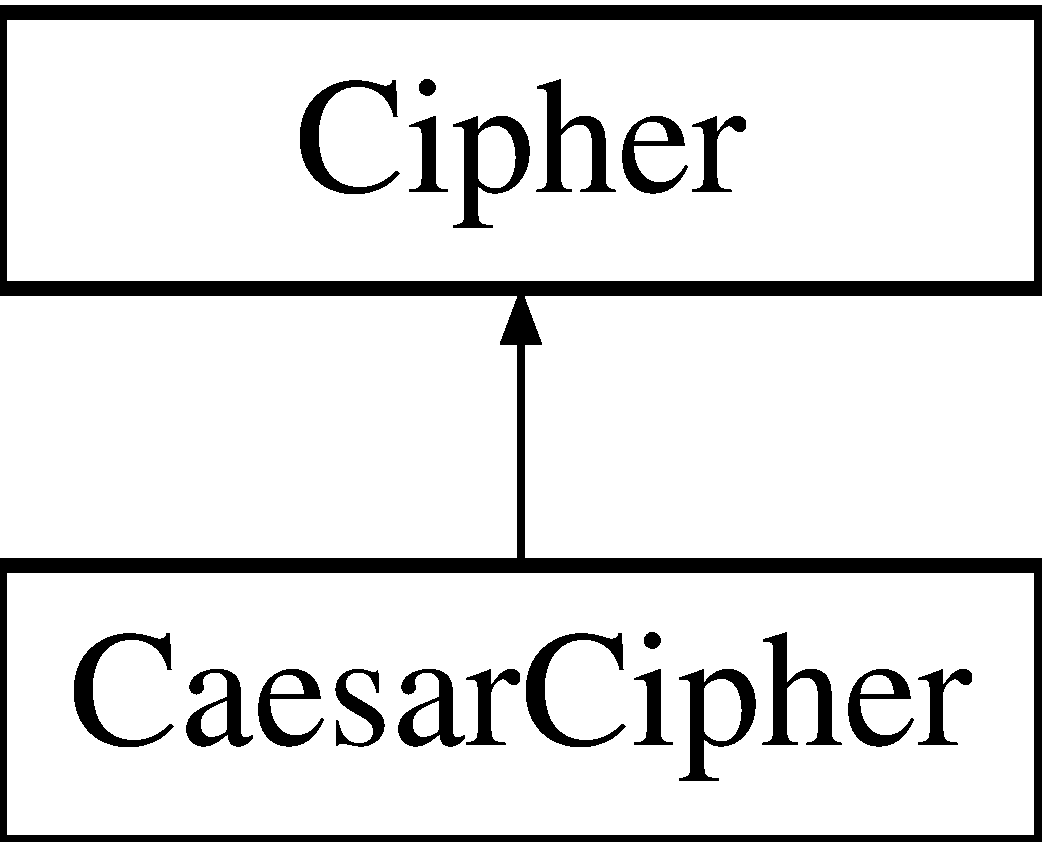
\includegraphics[height=2.000000cm]{class_caesar_cipher}
\end{center}
\end{figure}
\subsection*{Public Member Functions}
\begin{DoxyCompactItemize}
\item 
\hyperlink{class_caesar_cipher_afd5bb88c0e74234e76ad96b12d902931}{Caesar\+Cipher} (const size\+\_\+t key)
\item 
\hyperlink{class_caesar_cipher_a041ad5a8ef2b9e064a72fe64c9a97f4f}{Caesar\+Cipher} (const std\+::string \&key)
\item 
virtual std\+::string \hyperlink{class_caesar_cipher_ad9c70da70e7c465189ab1750e97fae5d}{apply\+Cipher} (const std\+::string \&input\+Text, const \hyperlink{_cipher_mode_8hpp_ac3adaabf9bad553901589ddf3de6daf5}{Cipher\+Mode} cipher\+Mode) const override
\end{DoxyCompactItemize}
\subsection*{Private Attributes}
\begin{DoxyCompactItemize}
\item 
size\+\_\+t \hyperlink{class_caesar_cipher_a7c29ddf093a91b51c91d977dcf57e7c3}{key\+\_\+} = 0\hypertarget{class_caesar_cipher_a7c29ddf093a91b51c91d977dcf57e7c3}{}\label{class_caesar_cipher_a7c29ddf093a91b51c91d977dcf57e7c3}

\begin{DoxyCompactList}\small\item\em The cipher key, essentially a constant shift to be applied. \end{DoxyCompactList}\end{DoxyCompactItemize}


\subsection{Detailed Description}
Encrypt or decrypt text using the Caesar cipher with the given key. 

\subsection{Constructor \& Destructor Documentation}
\index{Caesar\+Cipher@{Caesar\+Cipher}!Caesar\+Cipher@{Caesar\+Cipher}}
\index{Caesar\+Cipher@{Caesar\+Cipher}!Caesar\+Cipher@{Caesar\+Cipher}}
\subsubsection[{\texorpdfstring{Caesar\+Cipher(const size\+\_\+t key)}{CaesarCipher(const size_t key)}}]{\setlength{\rightskip}{0pt plus 5cm}Caesar\+Cipher\+::\+Caesar\+Cipher (
\begin{DoxyParamCaption}
\item[{const size\+\_\+t}]{key}
\end{DoxyParamCaption}
)\hspace{0.3cm}{\ttfamily [explicit]}}\hypertarget{class_caesar_cipher_afd5bb88c0e74234e76ad96b12d902931}{}\label{class_caesar_cipher_afd5bb88c0e74234e76ad96b12d902931}
Create a new \hyperlink{class_caesar_cipher}{Caesar\+Cipher} with the given key


\begin{DoxyParams}{Parameters}
{\em key} & the key to use in the cipher \\
\hline
\end{DoxyParams}
\index{Caesar\+Cipher@{Caesar\+Cipher}!Caesar\+Cipher@{Caesar\+Cipher}}
\index{Caesar\+Cipher@{Caesar\+Cipher}!Caesar\+Cipher@{Caesar\+Cipher}}
\subsubsection[{\texorpdfstring{Caesar\+Cipher(const std\+::string \&key)}{CaesarCipher(const std::string &key)}}]{\setlength{\rightskip}{0pt plus 5cm}Caesar\+Cipher\+::\+Caesar\+Cipher (
\begin{DoxyParamCaption}
\item[{const std\+::string \&}]{key}
\end{DoxyParamCaption}
)\hspace{0.3cm}{\ttfamily [explicit]}}\hypertarget{class_caesar_cipher_a041ad5a8ef2b9e064a72fe64c9a97f4f}{}\label{class_caesar_cipher_a041ad5a8ef2b9e064a72fe64c9a97f4f}
Create a new \hyperlink{class_caesar_cipher}{Caesar\+Cipher}, converting the given string into the key


\begin{DoxyParams}{Parameters}
{\em key} & the string to convert into the key to be used in the cipher \\
\hline
\end{DoxyParams}


\subsection{Member Function Documentation}
\index{Caesar\+Cipher@{Caesar\+Cipher}!apply\+Cipher@{apply\+Cipher}}
\index{apply\+Cipher@{apply\+Cipher}!Caesar\+Cipher@{Caesar\+Cipher}}
\subsubsection[{\texorpdfstring{apply\+Cipher(const std\+::string \&input\+Text, const Cipher\+Mode cipher\+Mode) const override}{applyCipher(const std::string &inputText, const CipherMode cipherMode) const override}}]{\setlength{\rightskip}{0pt plus 5cm}std\+::string Caesar\+Cipher\+::apply\+Cipher (
\begin{DoxyParamCaption}
\item[{const std\+::string \&}]{input\+Text, }
\item[{const {\bf Cipher\+Mode}}]{cipher\+Mode}
\end{DoxyParamCaption}
) const\hspace{0.3cm}{\ttfamily [override]}, {\ttfamily [virtual]}}\hypertarget{class_caesar_cipher_ad9c70da70e7c465189ab1750e97fae5d}{}\label{class_caesar_cipher_ad9c70da70e7c465189ab1750e97fae5d}
Apply the cipher to the provided text


\begin{DoxyParams}{Parameters}
{\em input\+Text} & the text to encrypt or decrypt \\
\hline
{\em cipher\+Mode} & whether to encrypt or decrypt the input text \\
\hline
\end{DoxyParams}
\begin{DoxyReturn}{Returns}
the result of applying the cipher to the input text 
\end{DoxyReturn}


Implements \hyperlink{class_cipher_ac6bbaa662c40483f3c0722109caf8572}{Cipher}.



The documentation for this class was generated from the following files\+:\begin{DoxyCompactItemize}
\item 
\hyperlink{_caesar_cipher_8hpp}{Caesar\+Cipher.\+hpp}\item 
Caesar\+Cipher.\+cpp\end{DoxyCompactItemize}

\hypertarget{class_cipher}{}\section{Cipher Class Reference}
\label{class_cipher}\index{Cipher@{Cipher}}


Defines the interface for a cipher.  




{\ttfamily \#include $<$M\+P\+A\+G\+S\+Cipher/\+Cipher.\+hpp$>$}

Inheritance diagram for Cipher\+:\begin{figure}[H]
\begin{center}
\leavevmode
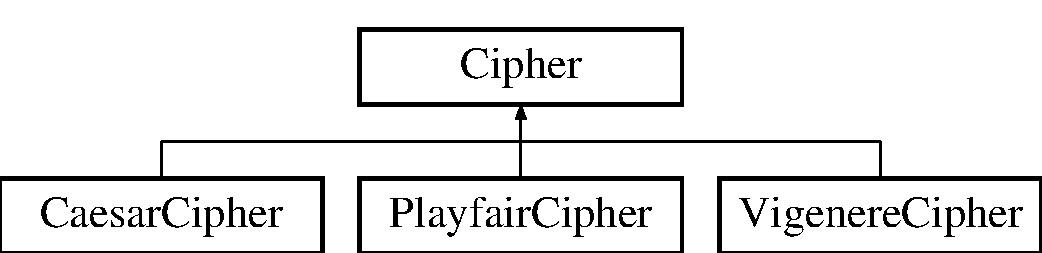
\includegraphics[height=2.000000cm]{class_cipher}
\end{center}
\end{figure}
\subsection*{Public Member Functions}
\begin{DoxyCompactItemize}
\item 
virtual std\+::string \hyperlink{class_cipher_ac6bbaa662c40483f3c0722109caf8572}{apply\+Cipher} (const std\+::string \&input\+Text, const \hyperlink{_cipher_mode_8hpp_ac3adaabf9bad553901589ddf3de6daf5}{Cipher\+Mode} cipher\+Mode) const =0
\item 
\hyperlink{class_cipher_a0f61b1dd7eb5a62d182cc7266600ff08}{Cipher} ()=default\hypertarget{class_cipher_a0f61b1dd7eb5a62d182cc7266600ff08}{}\label{class_cipher_a0f61b1dd7eb5a62d182cc7266600ff08}

\begin{DoxyCompactList}\small\item\em Default constructor. \end{DoxyCompactList}\item 
\hyperlink{class_cipher_a62a7b56af4d11ab44cbdb701adf6b3ea}{Cipher} (const \hyperlink{class_cipher}{Cipher} \&rhs)=default\hypertarget{class_cipher_a62a7b56af4d11ab44cbdb701adf6b3ea}{}\label{class_cipher_a62a7b56af4d11ab44cbdb701adf6b3ea}

\begin{DoxyCompactList}\small\item\em Default copy constructor. \end{DoxyCompactList}\item 
\hyperlink{class_cipher_a4ec5184e4bada371aebcca06cb3725ff}{Cipher} (\hyperlink{class_cipher}{Cipher} \&\&rhs)=default\hypertarget{class_cipher_a4ec5184e4bada371aebcca06cb3725ff}{}\label{class_cipher_a4ec5184e4bada371aebcca06cb3725ff}

\begin{DoxyCompactList}\small\item\em Default move constructor. \end{DoxyCompactList}\item 
\hyperlink{class_cipher}{Cipher} \& \hyperlink{class_cipher_ada389c6da626cade301d7b0ef5a5a22b}{operator=} (const \hyperlink{class_cipher}{Cipher} \&rhs)=default\hypertarget{class_cipher_ada389c6da626cade301d7b0ef5a5a22b}{}\label{class_cipher_ada389c6da626cade301d7b0ef5a5a22b}

\begin{DoxyCompactList}\small\item\em Default copy assignment operator. \end{DoxyCompactList}\item 
\hyperlink{class_cipher}{Cipher} \& \hyperlink{class_cipher_af0def19925ad32238ca0d7a74a90f115}{operator=} (\hyperlink{class_cipher}{Cipher} \&\&rhs)=default\hypertarget{class_cipher_af0def19925ad32238ca0d7a74a90f115}{}\label{class_cipher_af0def19925ad32238ca0d7a74a90f115}

\begin{DoxyCompactList}\small\item\em Default move assignment operator. \end{DoxyCompactList}\item 
virtual \hyperlink{class_cipher_af150a3783e81d40ded595b4c9e751b95}{$\sim$\+Cipher} ()=default\hypertarget{class_cipher_af150a3783e81d40ded595b4c9e751b95}{}\label{class_cipher_af150a3783e81d40ded595b4c9e751b95}

\begin{DoxyCompactList}\small\item\em Make the default destructor virtual. \end{DoxyCompactList}\end{DoxyCompactItemize}


\subsection{Detailed Description}
Defines the interface for a cipher. 

A purely abstract base class that defines the interface for a cipher

It can be used as follows\+: 
\begin{DoxyCode}
\textcolor{keyword}{class }MyCipher : \textcolor{keyword}{public} \hyperlink{class_cipher}{Cipher} \{...\};
\end{DoxyCode}
 

\subsection{Member Function Documentation}
\index{Cipher@{Cipher}!apply\+Cipher@{apply\+Cipher}}
\index{apply\+Cipher@{apply\+Cipher}!Cipher@{Cipher}}
\subsubsection[{\texorpdfstring{apply\+Cipher(const std\+::string \&input\+Text, const Cipher\+Mode cipher\+Mode) const =0}{applyCipher(const std::string &inputText, const CipherMode cipherMode) const =0}}]{\setlength{\rightskip}{0pt plus 5cm}virtual std\+::string Cipher\+::apply\+Cipher (
\begin{DoxyParamCaption}
\item[{const std\+::string \&}]{input\+Text, }
\item[{const {\bf Cipher\+Mode}}]{cipher\+Mode}
\end{DoxyParamCaption}
) const\hspace{0.3cm}{\ttfamily [pure virtual]}}\hypertarget{class_cipher_ac6bbaa662c40483f3c0722109caf8572}{}\label{class_cipher_ac6bbaa662c40483f3c0722109caf8572}
Apply the cipher to the provided text


\begin{DoxyParams}{Parameters}
{\em input\+Text} & the text to encrypt or decrypt \\
\hline
{\em cipher\+Mode} & whether to encrypt or decrypt the input text \\
\hline
\end{DoxyParams}
\begin{DoxyReturn}{Returns}
the result of applying the cipher to the input text 
\end{DoxyReturn}


Implemented in \hyperlink{class_vigenere_cipher_ad302e0a368a7f61368f0cfa894bdb792}{Vigenere\+Cipher}, \hyperlink{class_caesar_cipher_ad9c70da70e7c465189ab1750e97fae5d}{Caesar\+Cipher}, and \hyperlink{class_playfair_cipher_ac5e23f02becb84cb26d89dadeed87b05}{Playfair\+Cipher}.



The documentation for this class was generated from the following file\+:\begin{DoxyCompactItemize}
\item 
\hyperlink{_cipher_8hpp}{Cipher.\+hpp}\end{DoxyCompactItemize}

\hypertarget{class_invalid_cipher}{}\section{Invalid\+Cipher Class Reference}
\label{class_invalid_cipher}\index{Invalid\+Cipher@{Invalid\+Cipher}}


Exception to be thrown if an un-\/implemented cipher is passed as an arguement.  




{\ttfamily \#include $<$M\+P\+A\+G\+S\+Cipher/\+M\+P\+A\+G\+S\+Exceptions.\+hpp$>$}

Inheritance diagram for Invalid\+Cipher\+:\begin{figure}[H]
\begin{center}
\leavevmode
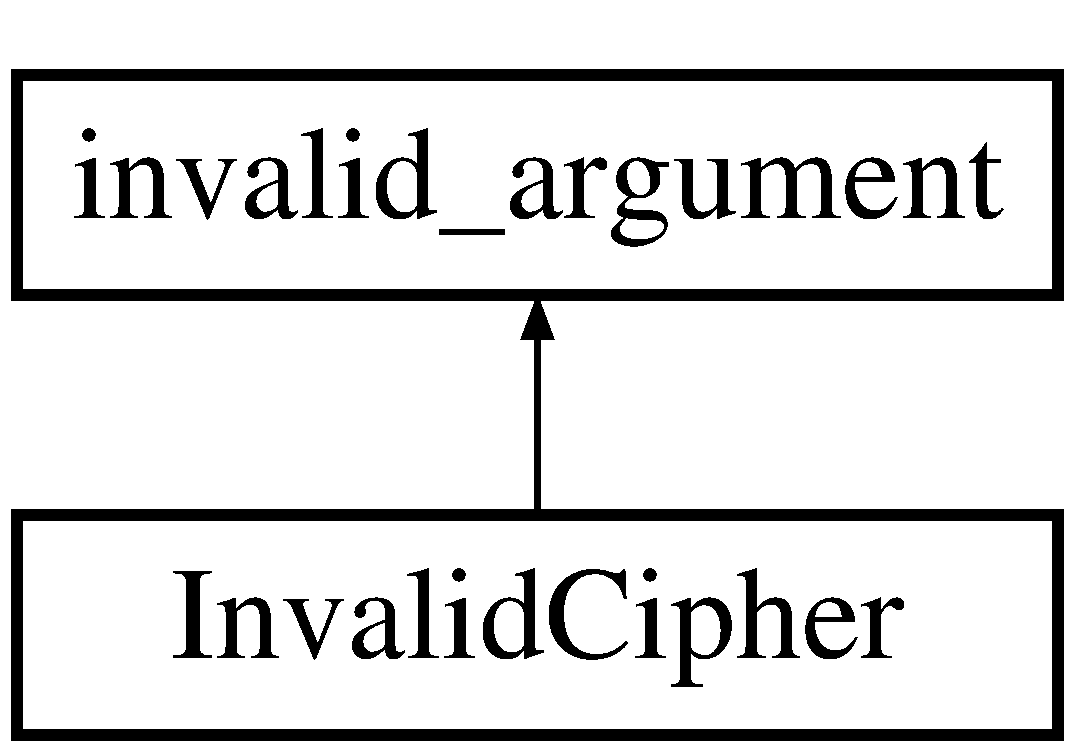
\includegraphics[height=2.000000cm]{class_invalid_cipher}
\end{center}
\end{figure}
\subsection*{Public Member Functions}
\begin{DoxyCompactItemize}
\item 
{\bfseries Invalid\+Cipher} (const std\+::string \&message)\hypertarget{class_invalid_cipher_abbc31aa58f5380031cd66c43a6aa7a37}{}\label{class_invalid_cipher_abbc31aa58f5380031cd66c43a6aa7a37}

\end{DoxyCompactItemize}


\subsection{Detailed Description}
Exception to be thrown if an un-\/implemented cipher is passed as an arguement. 


\begin{DoxyParams}{Parameters}
{\em message} & the message to be printed on raising \\
\hline
\end{DoxyParams}


The documentation for this class was generated from the following file\+:\begin{DoxyCompactItemize}
\item 
M\+P\+A\+G\+S\+Exceptions.\+hpp\end{DoxyCompactItemize}

\hypertarget{class_invalid_key}{}\section{Invalid\+Key Class Reference}
\label{class_invalid_key}\index{Invalid\+Key@{Invalid\+Key}}
Inheritance diagram for Invalid\+Key\+:\begin{figure}[H]
\begin{center}
\leavevmode
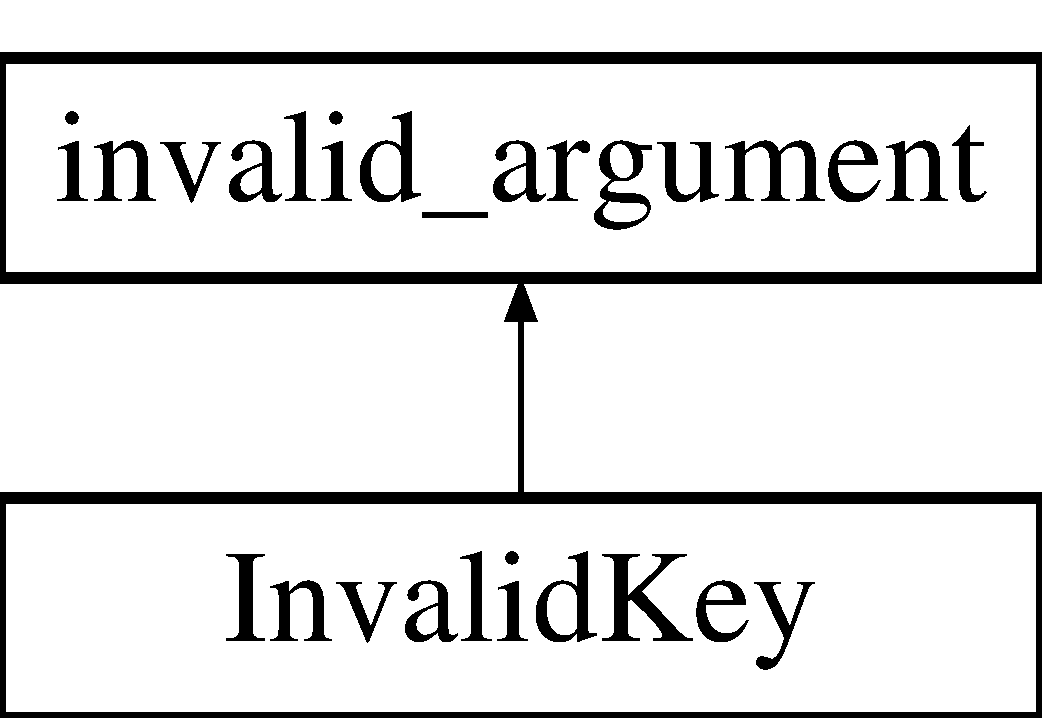
\includegraphics[height=2.000000cm]{class_invalid_key}
\end{center}
\end{figure}
\subsection*{Public Member Functions}
\begin{DoxyCompactItemize}
\item 
{\bfseries Invalid\+Key} (const std\+::string \&message)\hypertarget{class_invalid_key_a0b3717945958a1fbe0ff504fa6212c92}{}\label{class_invalid_key_a0b3717945958a1fbe0ff504fa6212c92}

\end{DoxyCompactItemize}


The documentation for this class was generated from the following file\+:\begin{DoxyCompactItemize}
\item 
M\+P\+A\+G\+S\+Exceptions.\+hpp\end{DoxyCompactItemize}

\hypertarget{class_missing_argument}{}\section{Missing\+Argument Class Reference}
\label{class_missing_argument}\index{Missing\+Argument@{Missing\+Argument}}


Exception to be thrown if a command line flag is not followed by the correct number of arguments.  




{\ttfamily \#include $<$M\+P\+A\+G\+S\+Cipher/\+M\+P\+A\+G\+S\+Exceptions.\+hpp$>$}

Inheritance diagram for Missing\+Argument\+:\begin{figure}[H]
\begin{center}
\leavevmode
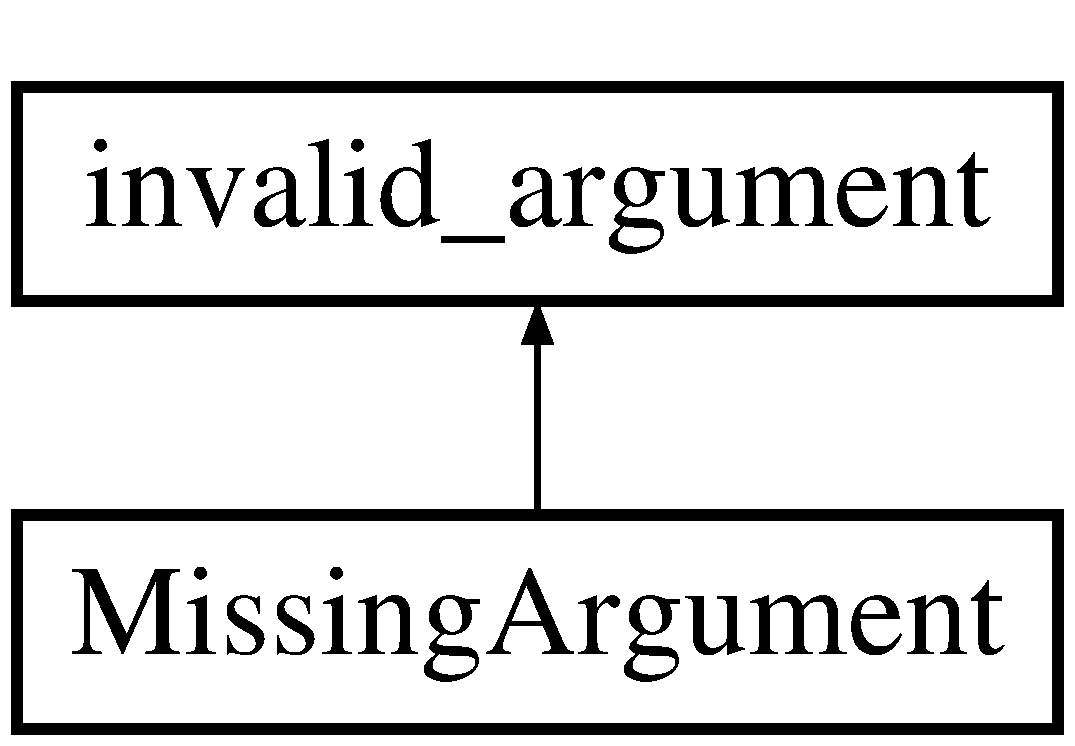
\includegraphics[height=2.000000cm]{class_missing_argument}
\end{center}
\end{figure}
\subsection*{Public Member Functions}
\begin{DoxyCompactItemize}
\item 
{\bfseries Missing\+Argument} (const std\+::string \&message)\hypertarget{class_missing_argument_a84ca3a1ba823eb806d1694b5f1fdb633}{}\label{class_missing_argument_a84ca3a1ba823eb806d1694b5f1fdb633}

\end{DoxyCompactItemize}


\subsection{Detailed Description}
Exception to be thrown if a command line flag is not followed by the correct number of arguments. 


\begin{DoxyParams}{Parameters}
{\em message} & the message to be printed on raising \\
\hline
\end{DoxyParams}


The documentation for this class was generated from the following file\+:\begin{DoxyCompactItemize}
\item 
M\+P\+A\+G\+S\+Exceptions.\+hpp\end{DoxyCompactItemize}

\hypertarget{class_playfair_cipher}{}\section{Playfair\+Cipher Class Reference}
\label{class_playfair_cipher}\index{Playfair\+Cipher@{Playfair\+Cipher}}


Encrypt or decrypt text using the Playfair cipher with the given key.  




{\ttfamily \#include $<$M\+P\+A\+G\+S\+Cipher/\+Playfair\+Cipher.\+hpp$>$}

Inheritance diagram for Playfair\+Cipher\+:\begin{figure}[H]
\begin{center}
\leavevmode
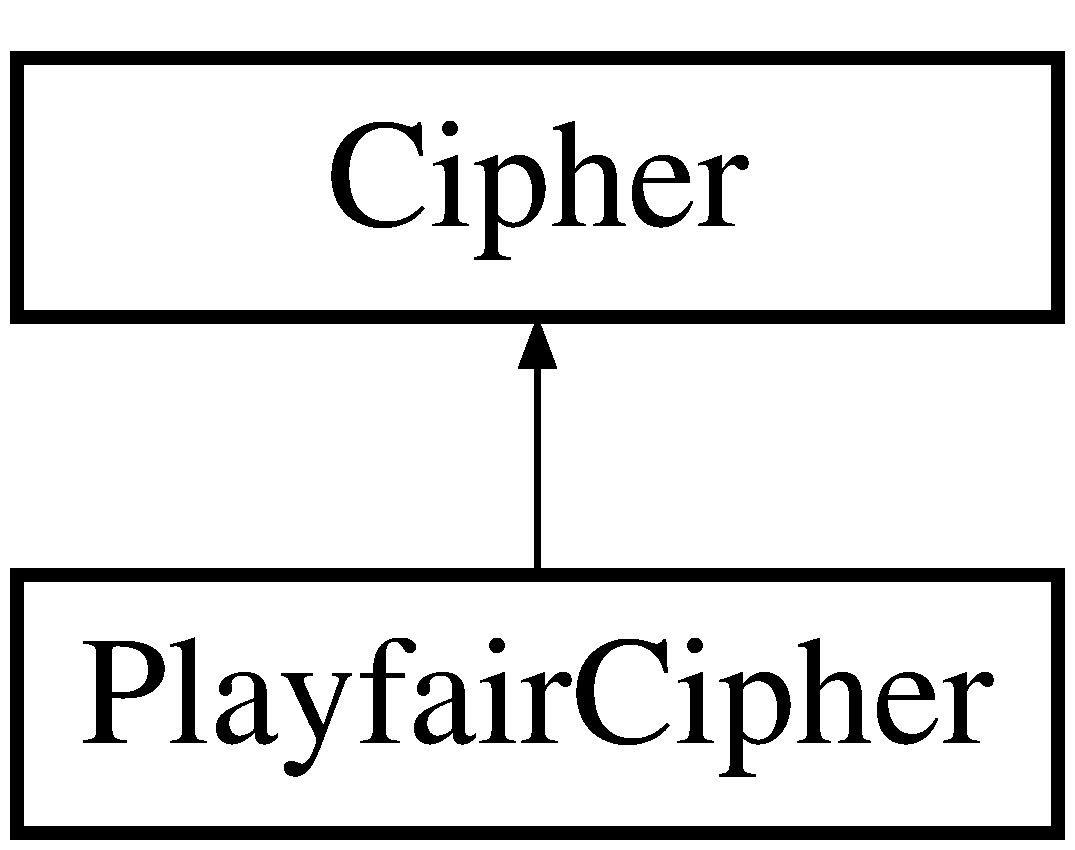
\includegraphics[height=2.000000cm]{class_playfair_cipher}
\end{center}
\end{figure}
\subsection*{Public Member Functions}
\begin{DoxyCompactItemize}
\item 
\hyperlink{class_playfair_cipher_abb71ab96f33cdcb0651c23f03952aef4}{Playfair\+Cipher} (const std\+::string \&key)
\item 
void \hyperlink{class_playfair_cipher_ab4a3d263f9101cb7aa50d4ad39c15737}{set\+Key} (const std\+::string \&key)
\item 
virtual std\+::string \hyperlink{class_playfair_cipher_ac5e23f02becb84cb26d89dadeed87b05}{apply\+Cipher} (const std\+::string \&input\+Text, const \hyperlink{_cipher_mode_8hpp_ac3adaabf9bad553901589ddf3de6daf5}{Cipher\+Mode} cipher\+Mode) const override
\end{DoxyCompactItemize}
\subsection*{Private Types}
\begin{DoxyCompactItemize}
\item 
using \hyperlink{class_playfair_cipher_a8e1ee213c8affc4e64fd29fd236a42ee}{Playfair\+Coords} = std\+::pair$<$ std\+::string\+::size\+\_\+type, std\+::string\+::size\+\_\+type $>$\hypertarget{class_playfair_cipher_a8e1ee213c8affc4e64fd29fd236a42ee}{}\label{class_playfair_cipher_a8e1ee213c8affc4e64fd29fd236a42ee}

\begin{DoxyCompactList}\small\item\em Type definition for the coordinates in the 5x5 table. \end{DoxyCompactList}\end{DoxyCompactItemize}
\subsection*{Private Attributes}
\begin{DoxyCompactItemize}
\item 
const std\+::string\+::size\+\_\+type \hyperlink{class_playfair_cipher_ae010f278b11579565f7166904d4c029a}{grid\+Dim\+\_\+} = 5\hypertarget{class_playfair_cipher_ae010f278b11579565f7166904d4c029a}{}\label{class_playfair_cipher_ae010f278b11579565f7166904d4c029a}

\begin{DoxyCompactList}\small\item\em The grid dimension. \end{DoxyCompactList}\item 
const std\+::string\+::size\+\_\+type \hyperlink{class_playfair_cipher_a1a3293fccc4e72fc1bd8e77142c6ae45}{key\+Length\+\_\+} = \hyperlink{class_playfair_cipher_ae010f278b11579565f7166904d4c029a}{grid\+Dim\+\_\+}$\ast$\hyperlink{class_playfair_cipher_ae010f278b11579565f7166904d4c029a}{grid\+Dim\+\_\+}\hypertarget{class_playfair_cipher_a1a3293fccc4e72fc1bd8e77142c6ae45}{}\label{class_playfair_cipher_a1a3293fccc4e72fc1bd8e77142c6ae45}

\begin{DoxyCompactList}\small\item\em The key length = grid dim$^\wedge$2. \end{DoxyCompactList}\item 
std\+::string \hyperlink{class_playfair_cipher_a4f7f68741424613b7200d3f34f963385}{key\+\_\+} = \char`\"{}\char`\"{}\hypertarget{class_playfair_cipher_a4f7f68741424613b7200d3f34f963385}{}\label{class_playfair_cipher_a4f7f68741424613b7200d3f34f963385}

\begin{DoxyCompactList}\small\item\em The cipher key. \end{DoxyCompactList}\item 
std\+::map$<$ char, \hyperlink{class_playfair_cipher_a8e1ee213c8affc4e64fd29fd236a42ee}{Playfair\+Coords} $>$ \hyperlink{class_playfair_cipher_a1e91611ed184fb0354a523efc6909724}{char\+Lookup\+\_\+}\hypertarget{class_playfair_cipher_a1e91611ed184fb0354a523efc6909724}{}\label{class_playfair_cipher_a1e91611ed184fb0354a523efc6909724}

\begin{DoxyCompactList}\small\item\em Lookup table to go from the character to the coordinates. \end{DoxyCompactList}\item 
std\+::map$<$ \hyperlink{class_playfair_cipher_a8e1ee213c8affc4e64fd29fd236a42ee}{Playfair\+Coords}, char $>$ \hyperlink{class_playfair_cipher_a1d772016641ca0ab178b25f24c996419}{coord\+Lookup\+\_\+}\hypertarget{class_playfair_cipher_a1d772016641ca0ab178b25f24c996419}{}\label{class_playfair_cipher_a1d772016641ca0ab178b25f24c996419}

\begin{DoxyCompactList}\small\item\em Lookup table to go from the coordinates to the character. \end{DoxyCompactList}\end{DoxyCompactItemize}


\subsection{Detailed Description}
Encrypt or decrypt text using the Playfair cipher with the given key. 

\subsection{Constructor \& Destructor Documentation}
\index{Playfair\+Cipher@{Playfair\+Cipher}!Playfair\+Cipher@{Playfair\+Cipher}}
\index{Playfair\+Cipher@{Playfair\+Cipher}!Playfair\+Cipher@{Playfair\+Cipher}}
\subsubsection[{\texorpdfstring{Playfair\+Cipher(const std\+::string \&key)}{PlayfairCipher(const std::string &key)}}]{\setlength{\rightskip}{0pt plus 5cm}Playfair\+Cipher\+::\+Playfair\+Cipher (
\begin{DoxyParamCaption}
\item[{const std\+::string \&}]{key}
\end{DoxyParamCaption}
)\hspace{0.3cm}{\ttfamily [explicit]}}\hypertarget{class_playfair_cipher_abb71ab96f33cdcb0651c23f03952aef4}{}\label{class_playfair_cipher_abb71ab96f33cdcb0651c23f03952aef4}
Create a new \hyperlink{class_playfair_cipher}{Playfair\+Cipher} with the given key


\begin{DoxyParams}{Parameters}
{\em key} & the key to use in the cipher \\
\hline
\end{DoxyParams}


\subsection{Member Function Documentation}
\index{Playfair\+Cipher@{Playfair\+Cipher}!apply\+Cipher@{apply\+Cipher}}
\index{apply\+Cipher@{apply\+Cipher}!Playfair\+Cipher@{Playfair\+Cipher}}
\subsubsection[{\texorpdfstring{apply\+Cipher(const std\+::string \&input\+Text, const Cipher\+Mode cipher\+Mode) const override}{applyCipher(const std::string &inputText, const CipherMode cipherMode) const override}}]{\setlength{\rightskip}{0pt plus 5cm}std\+::string Playfair\+Cipher\+::apply\+Cipher (
\begin{DoxyParamCaption}
\item[{const std\+::string \&}]{input\+Text, }
\item[{const {\bf Cipher\+Mode}}]{cipher\+Mode}
\end{DoxyParamCaption}
) const\hspace{0.3cm}{\ttfamily [override]}, {\ttfamily [virtual]}}\hypertarget{class_playfair_cipher_ac5e23f02becb84cb26d89dadeed87b05}{}\label{class_playfair_cipher_ac5e23f02becb84cb26d89dadeed87b05}
Apply the cipher to the provided text


\begin{DoxyParams}{Parameters}
{\em input\+Text} & the text to encrypt or decrypt \\
\hline
{\em cipher\+Mode} & whether to encrypt or decrypt the input text \\
\hline
\end{DoxyParams}
\begin{DoxyReturn}{Returns}
the result of applying the cipher to the input text 
\end{DoxyReturn}


Implements \hyperlink{class_cipher_ac6bbaa662c40483f3c0722109caf8572}{Cipher}.

\index{Playfair\+Cipher@{Playfair\+Cipher}!set\+Key@{set\+Key}}
\index{set\+Key@{set\+Key}!Playfair\+Cipher@{Playfair\+Cipher}}
\subsubsection[{\texorpdfstring{set\+Key(const std\+::string \&key)}{setKey(const std::string &key)}}]{\setlength{\rightskip}{0pt plus 5cm}void Playfair\+Cipher\+::set\+Key (
\begin{DoxyParamCaption}
\item[{const std\+::string \&}]{key}
\end{DoxyParamCaption}
)}\hypertarget{class_playfair_cipher_ab4a3d263f9101cb7aa50d4ad39c15737}{}\label{class_playfair_cipher_ab4a3d263f9101cb7aa50d4ad39c15737}
Set the key to be used for the encryption/decryption


\begin{DoxyParams}{Parameters}
{\em key} & the key to use in the cipher \\
\hline
\end{DoxyParams}


The documentation for this class was generated from the following files\+:\begin{DoxyCompactItemize}
\item 
\hyperlink{_playfair_cipher_8hpp}{Playfair\+Cipher.\+hpp}\item 
Playfair\+Cipher.\+cpp\end{DoxyCompactItemize}

\hypertarget{struct_program_settings}{}\section{Program\+Settings Struct Reference}
\label{struct_program_settings}\index{Program\+Settings@{Program\+Settings}}


Holds the settings of the program that can be modified by command-\/line arguments.  




{\ttfamily \#include $<$M\+P\+A\+G\+S\+Cipher/\+Process\+Command\+Line.\+hpp$>$}

\subsection*{Public Attributes}
\begin{DoxyCompactItemize}
\item 
bool \hyperlink{struct_program_settings_a2fa879c1b9330ffe56dfc05d1afeccf4}{help\+Requested}\hypertarget{struct_program_settings_a2fa879c1b9330ffe56dfc05d1afeccf4}{}\label{struct_program_settings_a2fa879c1b9330ffe56dfc05d1afeccf4}

\begin{DoxyCompactList}\small\item\em Indicates the presence of the help flag in the arguments. \end{DoxyCompactList}\item 
bool \hyperlink{struct_program_settings_a04ebebe91dad8638b8a85764241c49d2}{version\+Requested}\hypertarget{struct_program_settings_a04ebebe91dad8638b8a85764241c49d2}{}\label{struct_program_settings_a04ebebe91dad8638b8a85764241c49d2}

\begin{DoxyCompactList}\small\item\em Indicates the presence of the version flag in the arguments. \end{DoxyCompactList}\item 
std\+::string \hyperlink{struct_program_settings_af5edd8a1d7dff14319f501215e7b7257}{input\+File}\hypertarget{struct_program_settings_af5edd8a1d7dff14319f501215e7b7257}{}\label{struct_program_settings_af5edd8a1d7dff14319f501215e7b7257}

\begin{DoxyCompactList}\small\item\em Name of the input file. \end{DoxyCompactList}\item 
std\+::string \hyperlink{struct_program_settings_ac2e1105ba31a41b09d72f183533b2538}{output\+File}\hypertarget{struct_program_settings_ac2e1105ba31a41b09d72f183533b2538}{}\label{struct_program_settings_ac2e1105ba31a41b09d72f183533b2538}

\begin{DoxyCompactList}\small\item\em Name of the output file. \end{DoxyCompactList}\item 
std\+::string \hyperlink{struct_program_settings_a7cd3d165c25f89a7a0ad5224309f4d49}{cipher\+Key}\hypertarget{struct_program_settings_a7cd3d165c25f89a7a0ad5224309f4d49}{}\label{struct_program_settings_a7cd3d165c25f89a7a0ad5224309f4d49}

\begin{DoxyCompactList}\small\item\em Key to be used in encrypting/decrypting routine. \end{DoxyCompactList}\item 
\hyperlink{_cipher_mode_8hpp_ac3adaabf9bad553901589ddf3de6daf5}{Cipher\+Mode} \hyperlink{struct_program_settings_a4c9d4e90e44af4698ded0be678b6fd46}{cipher\+Mode}\hypertarget{struct_program_settings_a4c9d4e90e44af4698ded0be678b6fd46}{}\label{struct_program_settings_a4c9d4e90e44af4698ded0be678b6fd46}

\begin{DoxyCompactList}\small\item\em Flag indicating the mode in which the cipher should run (i.\+e. encrypt or decrypt) \end{DoxyCompactList}\item 
\hyperlink{_cipher_type_8hpp_aa1792f73cc3a05b7816d502879582348}{Cipher\+Type} \hyperlink{struct_program_settings_a01a75038fbb1c674e6fc3b6d36bf306e}{cipher\+Type}\hypertarget{struct_program_settings_a01a75038fbb1c674e6fc3b6d36bf306e}{}\label{struct_program_settings_a01a75038fbb1c674e6fc3b6d36bf306e}

\begin{DoxyCompactList}\small\item\em Flag to indicate which cipher to use (e.\+g. Caesar, Playfair, etc.) \end{DoxyCompactList}\end{DoxyCompactItemize}


\subsection{Detailed Description}
Holds the settings of the program that can be modified by command-\/line arguments. 

The documentation for this struct was generated from the following file\+:\begin{DoxyCompactItemize}
\item 
\hyperlink{_process_command_line_8hpp}{Process\+Command\+Line.\+hpp}\end{DoxyCompactItemize}

\hypertarget{class_unknown_argument}{}\section{Unknown\+Argument Class Reference}
\label{class_unknown_argument}\index{Unknown\+Argument@{Unknown\+Argument}}
Inheritance diagram for Unknown\+Argument\+:\begin{figure}[H]
\begin{center}
\leavevmode
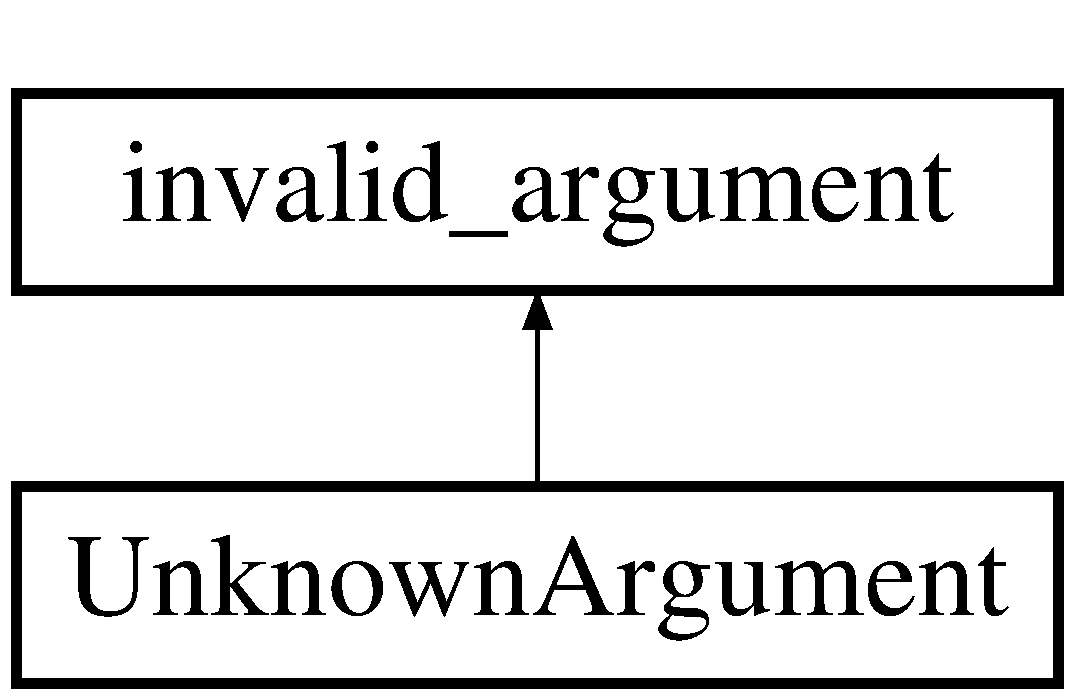
\includegraphics[height=2.000000cm]{class_unknown_argument}
\end{center}
\end{figure}
\subsection*{Public Member Functions}
\begin{DoxyCompactItemize}
\item 
{\bfseries Unknown\+Argument} (const std\+::string \&message)\hypertarget{class_unknown_argument_a43abeea9d1e4b257b2f8ff6528a5f081}{}\label{class_unknown_argument_a43abeea9d1e4b257b2f8ff6528a5f081}

\end{DoxyCompactItemize}


The documentation for this class was generated from the following file\+:\begin{DoxyCompactItemize}
\item 
M\+P\+A\+G\+S\+Exceptions.\+hpp\end{DoxyCompactItemize}

\hypertarget{class_vigenere_cipher}{}\section{Vigenere\+Cipher Class Reference}
\label{class_vigenere_cipher}\index{Vigenere\+Cipher@{Vigenere\+Cipher}}


Encrypt or decrypt text using the Vigenere cipher with the given key.  




{\ttfamily \#include $<$M\+P\+A\+G\+S\+Cipher/\+Vigenere\+Cipher.\+hpp$>$}

Inheritance diagram for Vigenere\+Cipher\+:\begin{figure}[H]
\begin{center}
\leavevmode
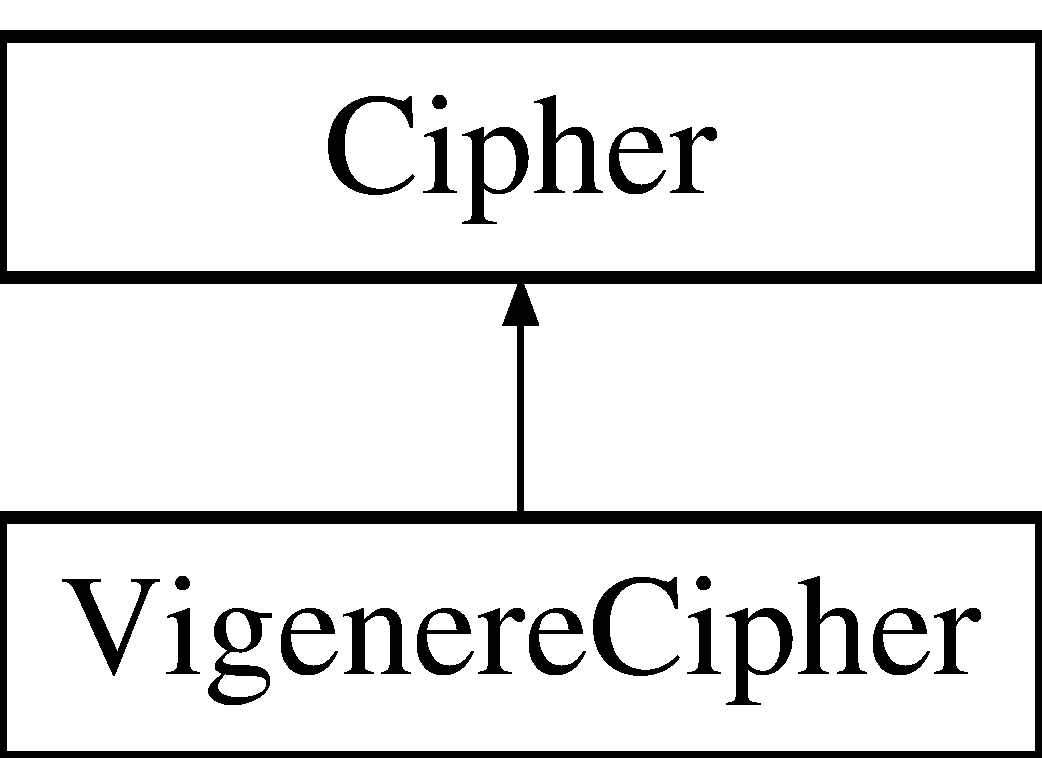
\includegraphics[height=2.000000cm]{class_vigenere_cipher}
\end{center}
\end{figure}
\subsection*{Public Member Functions}
\begin{DoxyCompactItemize}
\item 
\hyperlink{class_vigenere_cipher_ae4366bd9c507300040c276aff2b4088d}{Vigenere\+Cipher} (const std\+::string \&key)
\item 
void \hyperlink{class_vigenere_cipher_aed849482cc1402979c20d4087e6ca807}{set\+Key} (const std\+::string \&key)
\item 
virtual std\+::string \hyperlink{class_vigenere_cipher_ad302e0a368a7f61368f0cfa894bdb792}{apply\+Cipher} (const std\+::string \&input\+Text, const \hyperlink{_cipher_mode_8hpp_ac3adaabf9bad553901589ddf3de6daf5}{Cipher\+Mode} cipher\+Mode) const override
\end{DoxyCompactItemize}
\subsection*{Private Attributes}
\begin{DoxyCompactItemize}
\item 
std\+::string \hyperlink{class_vigenere_cipher_a834c19db11d2c93b25746b5a47b84342}{key\+\_\+} = \char`\"{}\char`\"{}\hypertarget{class_vigenere_cipher_a834c19db11d2c93b25746b5a47b84342}{}\label{class_vigenere_cipher_a834c19db11d2c93b25746b5a47b84342}

\begin{DoxyCompactList}\small\item\em The cipher key. \end{DoxyCompactList}\item 
std\+::map$<$ char, \hyperlink{class_caesar_cipher}{Caesar\+Cipher} $>$ \hyperlink{class_vigenere_cipher_ae710244c3caee93b8738e56aec26dcb9}{char\+Lookup\+\_\+}\hypertarget{class_vigenere_cipher_ae710244c3caee93b8738e56aec26dcb9}{}\label{class_vigenere_cipher_ae710244c3caee93b8738e56aec26dcb9}

\begin{DoxyCompactList}\small\item\em Lookup table to go from the character to the corresponding Caesar cipher. \end{DoxyCompactList}\end{DoxyCompactItemize}


\subsection{Detailed Description}
Encrypt or decrypt text using the Vigenere cipher with the given key. 

\subsection{Constructor \& Destructor Documentation}
\index{Vigenere\+Cipher@{Vigenere\+Cipher}!Vigenere\+Cipher@{Vigenere\+Cipher}}
\index{Vigenere\+Cipher@{Vigenere\+Cipher}!Vigenere\+Cipher@{Vigenere\+Cipher}}
\subsubsection[{\texorpdfstring{Vigenere\+Cipher(const std\+::string \&key)}{VigenereCipher(const std::string &key)}}]{\setlength{\rightskip}{0pt plus 5cm}Vigenere\+Cipher\+::\+Vigenere\+Cipher (
\begin{DoxyParamCaption}
\item[{const std\+::string \&}]{key}
\end{DoxyParamCaption}
)\hspace{0.3cm}{\ttfamily [explicit]}}\hypertarget{class_vigenere_cipher_ae4366bd9c507300040c276aff2b4088d}{}\label{class_vigenere_cipher_ae4366bd9c507300040c276aff2b4088d}
Create a new \hyperlink{class_vigenere_cipher}{Vigenere\+Cipher} with the given key


\begin{DoxyParams}{Parameters}
{\em key} & the key to use in the cipher \\
\hline
\end{DoxyParams}


\subsection{Member Function Documentation}
\index{Vigenere\+Cipher@{Vigenere\+Cipher}!apply\+Cipher@{apply\+Cipher}}
\index{apply\+Cipher@{apply\+Cipher}!Vigenere\+Cipher@{Vigenere\+Cipher}}
\subsubsection[{\texorpdfstring{apply\+Cipher(const std\+::string \&input\+Text, const Cipher\+Mode cipher\+Mode) const override}{applyCipher(const std::string &inputText, const CipherMode cipherMode) const override}}]{\setlength{\rightskip}{0pt plus 5cm}std\+::string Vigenere\+Cipher\+::apply\+Cipher (
\begin{DoxyParamCaption}
\item[{const std\+::string \&}]{input\+Text, }
\item[{const {\bf Cipher\+Mode}}]{cipher\+Mode}
\end{DoxyParamCaption}
) const\hspace{0.3cm}{\ttfamily [override]}, {\ttfamily [virtual]}}\hypertarget{class_vigenere_cipher_ad302e0a368a7f61368f0cfa894bdb792}{}\label{class_vigenere_cipher_ad302e0a368a7f61368f0cfa894bdb792}
Apply the cipher to the provided text


\begin{DoxyParams}{Parameters}
{\em input\+Text} & the text to encrypt or decrypt \\
\hline
{\em cipher\+Mode} & whether to encrypt or decrypt the input text \\
\hline
\end{DoxyParams}
\begin{DoxyReturn}{Returns}
the result of applying the cipher to the input text 
\end{DoxyReturn}


Implements \hyperlink{class_cipher_ac6bbaa662c40483f3c0722109caf8572}{Cipher}.

\index{Vigenere\+Cipher@{Vigenere\+Cipher}!set\+Key@{set\+Key}}
\index{set\+Key@{set\+Key}!Vigenere\+Cipher@{Vigenere\+Cipher}}
\subsubsection[{\texorpdfstring{set\+Key(const std\+::string \&key)}{setKey(const std::string &key)}}]{\setlength{\rightskip}{0pt plus 5cm}void Vigenere\+Cipher\+::set\+Key (
\begin{DoxyParamCaption}
\item[{const std\+::string \&}]{key}
\end{DoxyParamCaption}
)}\hypertarget{class_vigenere_cipher_aed849482cc1402979c20d4087e6ca807}{}\label{class_vigenere_cipher_aed849482cc1402979c20d4087e6ca807}
Set the key to be used for the encryption/decryption


\begin{DoxyParams}{Parameters}
{\em key} & the key to use in the cipher \\
\hline
\end{DoxyParams}


The documentation for this class was generated from the following files\+:\begin{DoxyCompactItemize}
\item 
\hyperlink{_vigenere_cipher_8hpp}{Vigenere\+Cipher.\+hpp}\item 
Vigenere\+Cipher.\+cpp\end{DoxyCompactItemize}

\chapter{File Documentation}
\hypertarget{_alphabet_8hpp}{}\section{Alphabet.\+hpp File Reference}
\label{_alphabet_8hpp}\index{Alphabet.\+hpp@{Alphabet.\+hpp}}


Contains the declaration of the \hyperlink{namespace_alphabet}{Alphabet} namespace, which holds various commonly used constants.  


\subsection*{Namespaces}
\begin{DoxyCompactItemize}
\item 
 \hyperlink{namespace_alphabet}{Alphabet}
\begin{DoxyCompactList}\small\item\em Namespace to hold alphabet-\/related constants. \end{DoxyCompactList}\end{DoxyCompactItemize}
\subsection*{Typedefs}
\begin{DoxyCompactItemize}
\item 
using \hyperlink{namespace_alphabet_a5b8e9bc01c32a14e85582df88cd8275a}{Alphabet\+::\+Alphabet\+Size} = std\+::string\+::size\+\_\+type\hypertarget{namespace_alphabet_a5b8e9bc01c32a14e85582df88cd8275a}{}\label{namespace_alphabet_a5b8e9bc01c32a14e85582df88cd8275a}

\begin{DoxyCompactList}\small\item\em The type that represents the size of the alphabet. \end{DoxyCompactList}\end{DoxyCompactItemize}
\subsection*{Variables}
\begin{DoxyCompactItemize}
\item 
const std\+::string \hyperlink{namespace_alphabet_a30996a14237b471696a3f11a3596fcbf}{Alphabet\+::alphabet} \{\char`\"{}A\+B\+C\+D\+E\+F\+G\+H\+I\+J\+K\+L\+M\+N\+O\+P\+Q\+R\+S\+T\+U\+V\+W\+X\+YZ\char`\"{}\}\hypertarget{namespace_alphabet_a30996a14237b471696a3f11a3596fcbf}{}\label{namespace_alphabet_a30996a14237b471696a3f11a3596fcbf}

\begin{DoxyCompactList}\small\item\em The alphabet. \end{DoxyCompactList}\item 
const Alphabet\+Size \hyperlink{namespace_alphabet_a756e45f4de2154e6d680f5e9f382363a}{Alphabet\+::size} \{ alphabet.\+size() \}\hypertarget{namespace_alphabet_a756e45f4de2154e6d680f5e9f382363a}{}\label{namespace_alphabet_a756e45f4de2154e6d680f5e9f382363a}

\begin{DoxyCompactList}\small\item\em The size of the alphabet. \end{DoxyCompactList}\end{DoxyCompactItemize}


\subsection{Detailed Description}
Contains the declaration of the \hyperlink{namespace_alphabet}{Alphabet} namespace, which holds various commonly used constants. 


\hypertarget{_caesar_cipher_8hpp}{}\section{Caesar\+Cipher.\+hpp File Reference}
\label{_caesar_cipher_8hpp}\index{Caesar\+Cipher.\+hpp@{Caesar\+Cipher.\+hpp}}


Contains the declaration of the \hyperlink{class_caesar_cipher}{Caesar\+Cipher} class.  


{\ttfamily \#include $<$string$>$}\\*
{\ttfamily \#include $<$vector$>$}\\*
{\ttfamily \#include \char`\"{}Cipher.\+hpp\char`\"{}}\\*
{\ttfamily \#include \char`\"{}Cipher\+Mode.\+hpp\char`\"{}}\\*
\subsection*{Classes}
\begin{DoxyCompactItemize}
\item 
class \hyperlink{class_caesar_cipher}{Caesar\+Cipher}
\begin{DoxyCompactList}\small\item\em Encrypt or decrypt text using the Caesar cipher with the given key. \end{DoxyCompactList}\end{DoxyCompactItemize}


\subsection{Detailed Description}
Contains the declaration of the \hyperlink{class_caesar_cipher}{Caesar\+Cipher} class. 


\hypertarget{_cipher_8hpp}{}\section{Cipher.\+hpp File Reference}
\label{_cipher_8hpp}\index{Cipher.\+hpp@{Cipher.\+hpp}}


Contains the declaration of the purely abstract \hyperlink{class_cipher}{Cipher} base class.  


{\ttfamily \#include $<$string$>$}\\*
{\ttfamily \#include \char`\"{}Cipher\+Mode.\+hpp\char`\"{}}\\*
\subsection*{Classes}
\begin{DoxyCompactItemize}
\item 
class \hyperlink{class_cipher}{Cipher}
\begin{DoxyCompactList}\small\item\em Defines the interface for a cipher. \end{DoxyCompactList}\end{DoxyCompactItemize}


\subsection{Detailed Description}
Contains the declaration of the purely abstract \hyperlink{class_cipher}{Cipher} base class. 


\hypertarget{_cipher_factory_8hpp}{}\section{Cipher\+Factory.\+hpp File Reference}
\label{_cipher_factory_8hpp}\index{Cipher\+Factory.\+hpp@{Cipher\+Factory.\+hpp}}


Contains the declaration of the factory function for creating \hyperlink{class_cipher}{Cipher} objects.  


{\ttfamily \#include $<$memory$>$}\\*
{\ttfamily \#include $<$string$>$}\\*
{\ttfamily \#include \char`\"{}Cipher.\+hpp\char`\"{}}\\*
{\ttfamily \#include \char`\"{}Cipher\+Type.\+hpp\char`\"{}}\\*
\subsection*{Functions}
\begin{DoxyCompactItemize}
\item 
std\+::unique\+\_\+ptr$<$ \hyperlink{class_cipher}{Cipher} $>$ \hyperlink{_cipher_factory_8hpp_a58dc798755cc2d37c965f3c2ef754e1c}{cipher\+Factory} (const \hyperlink{_cipher_type_8hpp_aa1792f73cc3a05b7816d502879582348}{Cipher\+Type} type, const std\+::string \&key)
\begin{DoxyCompactList}\small\item\em Create a \hyperlink{class_cipher}{Cipher} object of the concrete type specified, constructed from the supplied key. \end{DoxyCompactList}\end{DoxyCompactItemize}


\subsection{Detailed Description}
Contains the declaration of the factory function for creating \hyperlink{class_cipher}{Cipher} objects. 



\subsection{Function Documentation}
\index{Cipher\+Factory.\+hpp@{Cipher\+Factory.\+hpp}!cipher\+Factory@{cipher\+Factory}}
\index{cipher\+Factory@{cipher\+Factory}!Cipher\+Factory.\+hpp@{Cipher\+Factory.\+hpp}}
\subsubsection[{\texorpdfstring{cipher\+Factory(const Cipher\+Type type, const std\+::string \&key)}{cipherFactory(const CipherType type, const std::string &key)}}]{\setlength{\rightskip}{0pt plus 5cm}std\+::unique\+\_\+ptr$<${\bf Cipher}$>$ cipher\+Factory (
\begin{DoxyParamCaption}
\item[{const {\bf Cipher\+Type}}]{type, }
\item[{const std\+::string \&}]{key}
\end{DoxyParamCaption}
)}\hypertarget{_cipher_factory_8hpp_a58dc798755cc2d37c965f3c2ef754e1c}{}\label{_cipher_factory_8hpp_a58dc798755cc2d37c965f3c2ef754e1c}


Create a \hyperlink{class_cipher}{Cipher} object of the concrete type specified, constructed from the supplied key. 


\begin{DoxyParams}{Parameters}
{\em type} & the concrete type of of cipher to be constructed \\
\hline
{\em key} & the key with which to construct the cipher \\
\hline
\end{DoxyParams}
\begin{DoxyReturn}{Returns}
the newly constructed cipher 
\end{DoxyReturn}

\hypertarget{_cipher_mode_8hpp}{}\section{Cipher\+Mode.\+hpp File Reference}
\label{_cipher_mode_8hpp}\index{Cipher\+Mode.\+hpp@{Cipher\+Mode.\+hpp}}


Contains the declaration of the Cipher\+Mode enumeration.  


\subsection*{Enumerations}
\begin{DoxyCompactItemize}
\item 
enum \hyperlink{_cipher_mode_8hpp_ac3adaabf9bad553901589ddf3de6daf5}{Cipher\+Mode} \{ \hyperlink{_cipher_mode_8hpp_ac3adaabf9bad553901589ddf3de6daf5a611d29c748a7931c825a247fcf3f290e}{Cipher\+Mode\+::\+Encrypt}, 
\hyperlink{_cipher_mode_8hpp_ac3adaabf9bad553901589ddf3de6daf5a762e3a77ecdd773da2b859e6807529a2}{Cipher\+Mode\+::\+Decrypt}
 \}\begin{DoxyCompactList}\small\item\em Enumeration to define the modes in which the ciphers can operate. \end{DoxyCompactList}
\end{DoxyCompactItemize}


\subsection{Detailed Description}
Contains the declaration of the Cipher\+Mode enumeration. 



\subsection{Enumeration Type Documentation}
\index{Cipher\+Mode.\+hpp@{Cipher\+Mode.\+hpp}!Cipher\+Mode@{Cipher\+Mode}}
\index{Cipher\+Mode@{Cipher\+Mode}!Cipher\+Mode.\+hpp@{Cipher\+Mode.\+hpp}}
\subsubsection[{\texorpdfstring{Cipher\+Mode}{CipherMode}}]{\setlength{\rightskip}{0pt plus 5cm}enum {\bf Cipher\+Mode}\hspace{0.3cm}{\ttfamily [strong]}}\hypertarget{_cipher_mode_8hpp_ac3adaabf9bad553901589ddf3de6daf5}{}\label{_cipher_mode_8hpp_ac3adaabf9bad553901589ddf3de6daf5}


Enumeration to define the modes in which the ciphers can operate. 

\begin{Desc}
\item[Enumerator]\par
\begin{description}
\index{Encrypt@{Encrypt}!Cipher\+Mode.\+hpp@{Cipher\+Mode.\+hpp}}\index{Cipher\+Mode.\+hpp@{Cipher\+Mode.\+hpp}!Encrypt@{Encrypt}}\item[{\em 
Encrypt\hypertarget{_cipher_mode_8hpp_ac3adaabf9bad553901589ddf3de6daf5a611d29c748a7931c825a247fcf3f290e}{}\label{_cipher_mode_8hpp_ac3adaabf9bad553901589ddf3de6daf5a611d29c748a7931c825a247fcf3f290e}
}]Apply cipher in encrypt mode. \index{Decrypt@{Decrypt}!Cipher\+Mode.\+hpp@{Cipher\+Mode.\+hpp}}\index{Cipher\+Mode.\+hpp@{Cipher\+Mode.\+hpp}!Decrypt@{Decrypt}}\item[{\em 
Decrypt\hypertarget{_cipher_mode_8hpp_ac3adaabf9bad553901589ddf3de6daf5a762e3a77ecdd773da2b859e6807529a2}{}\label{_cipher_mode_8hpp_ac3adaabf9bad553901589ddf3de6daf5a762e3a77ecdd773da2b859e6807529a2}
}]Apply cipher in decrypt mode. \end{description}
\end{Desc}

\hypertarget{_cipher_type_8hpp}{}\section{Cipher\+Type.\+hpp File Reference}
\label{_cipher_type_8hpp}\index{Cipher\+Type.\+hpp@{Cipher\+Type.\+hpp}}


Contains the declaration of the Cipher\+Type enumeration.  


\subsection*{Enumerations}
\begin{DoxyCompactItemize}
\item 
enum \hyperlink{_cipher_type_8hpp_aa1792f73cc3a05b7816d502879582348}{Cipher\+Type} \{ \hyperlink{_cipher_type_8hpp_aa1792f73cc3a05b7816d502879582348a6d086db90583fcea884ecf10f2dc6319}{Cipher\+Type\+::\+Caesar}, 
\hyperlink{_cipher_type_8hpp_aa1792f73cc3a05b7816d502879582348aa6a466d0a4f7cabf3afcc5d466c1c78c}{Cipher\+Type\+::\+Playfair}, 
\hyperlink{_cipher_type_8hpp_aa1792f73cc3a05b7816d502879582348ac933404dc8484a4f3f2b79cfd0bc2474}{Cipher\+Type\+::\+Vigenere}
 \}\begin{DoxyCompactList}\small\item\em Enumeration to define the ciphers that can be used. \end{DoxyCompactList}
\end{DoxyCompactItemize}


\subsection{Detailed Description}
Contains the declaration of the Cipher\+Type enumeration. 



\subsection{Enumeration Type Documentation}
\index{Cipher\+Type.\+hpp@{Cipher\+Type.\+hpp}!Cipher\+Type@{Cipher\+Type}}
\index{Cipher\+Type@{Cipher\+Type}!Cipher\+Type.\+hpp@{Cipher\+Type.\+hpp}}
\subsubsection[{\texorpdfstring{Cipher\+Type}{CipherType}}]{\setlength{\rightskip}{0pt plus 5cm}enum {\bf Cipher\+Type}\hspace{0.3cm}{\ttfamily [strong]}}\hypertarget{_cipher_type_8hpp_aa1792f73cc3a05b7816d502879582348}{}\label{_cipher_type_8hpp_aa1792f73cc3a05b7816d502879582348}


Enumeration to define the ciphers that can be used. 

\begin{Desc}
\item[Enumerator]\par
\begin{description}
\index{Caesar@{Caesar}!Cipher\+Type.\+hpp@{Cipher\+Type.\+hpp}}\index{Cipher\+Type.\+hpp@{Cipher\+Type.\+hpp}!Caesar@{Caesar}}\item[{\em 
Caesar\hypertarget{_cipher_type_8hpp_aa1792f73cc3a05b7816d502879582348a6d086db90583fcea884ecf10f2dc6319}{}\label{_cipher_type_8hpp_aa1792f73cc3a05b7816d502879582348a6d086db90583fcea884ecf10f2dc6319}
}]The Caesar cipher. \index{Playfair@{Playfair}!Cipher\+Type.\+hpp@{Cipher\+Type.\+hpp}}\index{Cipher\+Type.\+hpp@{Cipher\+Type.\+hpp}!Playfair@{Playfair}}\item[{\em 
Playfair\hypertarget{_cipher_type_8hpp_aa1792f73cc3a05b7816d502879582348aa6a466d0a4f7cabf3afcc5d466c1c78c}{}\label{_cipher_type_8hpp_aa1792f73cc3a05b7816d502879582348aa6a466d0a4f7cabf3afcc5d466c1c78c}
}]The Playfair cipher. \index{Vigenere@{Vigenere}!Cipher\+Type.\+hpp@{Cipher\+Type.\+hpp}}\index{Cipher\+Type.\+hpp@{Cipher\+Type.\+hpp}!Vigenere@{Vigenere}}\item[{\em 
Vigenere\hypertarget{_cipher_type_8hpp_aa1792f73cc3a05b7816d502879582348ac933404dc8484a4f3f2b79cfd0bc2474}{}\label{_cipher_type_8hpp_aa1792f73cc3a05b7816d502879582348ac933404dc8484a4f3f2b79cfd0bc2474}
}]The Vigenere cipher. \end{description}
\end{Desc}

\hypertarget{_playfair_cipher_8hpp}{}\section{Playfair\+Cipher.\+hpp File Reference}
\label{_playfair_cipher_8hpp}\index{Playfair\+Cipher.\+hpp@{Playfair\+Cipher.\+hpp}}


Contains the declaration of the \hyperlink{class_playfair_cipher}{Playfair\+Cipher} class.  


{\ttfamily \#include $<$string$>$}\\*
{\ttfamily \#include $<$map$>$}\\*
{\ttfamily \#include \char`\"{}Cipher.\+hpp\char`\"{}}\\*
{\ttfamily \#include \char`\"{}Cipher\+Mode.\+hpp\char`\"{}}\\*
\subsection*{Classes}
\begin{DoxyCompactItemize}
\item 
class \hyperlink{class_playfair_cipher}{Playfair\+Cipher}
\begin{DoxyCompactList}\small\item\em Encrypt or decrypt text using the Playfair cipher with the given key. \end{DoxyCompactList}\end{DoxyCompactItemize}


\subsection{Detailed Description}
Contains the declaration of the \hyperlink{class_playfair_cipher}{Playfair\+Cipher} class. 


\hypertarget{_process_command_line_8hpp}{}\section{Process\+Command\+Line.\+hpp File Reference}
\label{_process_command_line_8hpp}\index{Process\+Command\+Line.\+hpp@{Process\+Command\+Line.\+hpp}}


Contains the declarations of the data structures and functions associated with the processing of command-\/line arguments.  


{\ttfamily \#include $<$string$>$}\\*
{\ttfamily \#include $<$vector$>$}\\*
{\ttfamily \#include \char`\"{}Cipher\+Mode.\+hpp\char`\"{}}\\*
{\ttfamily \#include \char`\"{}Cipher\+Type.\+hpp\char`\"{}}\\*
\subsection*{Classes}
\begin{DoxyCompactItemize}
\item 
struct \hyperlink{struct_program_settings}{Program\+Settings}
\begin{DoxyCompactList}\small\item\em Holds the settings of the program that can be modified by command-\/line arguments. \end{DoxyCompactList}\end{DoxyCompactItemize}
\subsection*{Functions}
\begin{DoxyCompactItemize}
\item 
void \hyperlink{_process_command_line_8hpp_af7f2f0960ef5ac4941e8fcb10138d772}{process\+Command\+Line} (const std\+::vector$<$ std\+::string $>$ \&args, \hyperlink{struct_program_settings}{Program\+Settings} \&settings)
\begin{DoxyCompactList}\small\item\em Processes the command-\/line arguments and modifies accordingly the program settings. \end{DoxyCompactList}\end{DoxyCompactItemize}


\subsection{Detailed Description}
Contains the declarations of the data structures and functions associated with the processing of command-\/line arguments. 



\subsection{Function Documentation}
\index{Process\+Command\+Line.\+hpp@{Process\+Command\+Line.\+hpp}!process\+Command\+Line@{process\+Command\+Line}}
\index{process\+Command\+Line@{process\+Command\+Line}!Process\+Command\+Line.\+hpp@{Process\+Command\+Line.\+hpp}}
\subsubsection[{\texorpdfstring{process\+Command\+Line(const std\+::vector$<$ std\+::string $>$ \&args, Program\+Settings \&settings)}{processCommandLine(const std::vector< std::string > &args, ProgramSettings &settings)}}]{\setlength{\rightskip}{0pt plus 5cm}void process\+Command\+Line (
\begin{DoxyParamCaption}
\item[{const std\+::vector$<$ std\+::string $>$ \&}]{args, }
\item[{{\bf Program\+Settings} \&}]{settings}
\end{DoxyParamCaption}
)}\hypertarget{_process_command_line_8hpp_af7f2f0960ef5ac4941e8fcb10138d772}{}\label{_process_command_line_8hpp_af7f2f0960ef5ac4941e8fcb10138d772}


Processes the command-\/line arguments and modifies accordingly the program settings. 


\begin{DoxyParams}{Parameters}
{\em args} & the command-\/line arguments to be processed \\
\hline
{\em settings} & the program settings to be modified based upon the arguments received \\
\hline
\end{DoxyParams}
\begin{DoxyReturn}{Returns}
true if the arguments could be successfully parsed, false otherwise 
\end{DoxyReturn}

\hypertarget{_transform_char_8hpp}{}\section{Transform\+Char.\+hpp File Reference}
\label{_transform_char_8hpp}\index{Transform\+Char.\+hpp@{Transform\+Char.\+hpp}}


Contains the declaration of the function for processing the input text.  


{\ttfamily \#include $<$string$>$}\\*
\subsection*{Functions}
\begin{DoxyCompactItemize}
\item 
std\+::string \hyperlink{_transform_char_8hpp_a4efd038e9b5e9b128fca12d8d321dead}{transform\+Char} (const char in)
\begin{DoxyCompactList}\small\item\em Transliterate char to string. \end{DoxyCompactList}\end{DoxyCompactItemize}


\subsection{Detailed Description}
Contains the declaration of the function for processing the input text. 



\subsection{Function Documentation}
\index{Transform\+Char.\+hpp@{Transform\+Char.\+hpp}!transform\+Char@{transform\+Char}}
\index{transform\+Char@{transform\+Char}!Transform\+Char.\+hpp@{Transform\+Char.\+hpp}}
\subsubsection[{\texorpdfstring{transform\+Char(const char in)}{transformChar(const char in)}}]{\setlength{\rightskip}{0pt plus 5cm}std\+::string transform\+Char (
\begin{DoxyParamCaption}
\item[{const char}]{in}
\end{DoxyParamCaption}
)}\hypertarget{_transform_char_8hpp_a4efd038e9b5e9b128fca12d8d321dead}{}\label{_transform_char_8hpp_a4efd038e9b5e9b128fca12d8d321dead}


Transliterate char to string. 

\hyperlink{namespace_alphabet}{Alphabet} characters are made uppercase Digits are replaced with their english word equivalents All other characters are discarded


\begin{DoxyParams}{Parameters}
{\em in} & the character to process \\
\hline
\end{DoxyParams}
\begin{DoxyReturn}{Returns}
the transliterated string 
\end{DoxyReturn}

\hypertarget{_vigenere_cipher_8hpp}{}\section{Vigenere\+Cipher.\+hpp File Reference}
\label{_vigenere_cipher_8hpp}\index{Vigenere\+Cipher.\+hpp@{Vigenere\+Cipher.\+hpp}}


Contains the declaration of the \hyperlink{class_vigenere_cipher}{Vigenere\+Cipher} class.  


{\ttfamily \#include $<$string$>$}\\*
{\ttfamily \#include $<$map$>$}\\*
{\ttfamily \#include \char`\"{}Cipher.\+hpp\char`\"{}}\\*
{\ttfamily \#include \char`\"{}Cipher\+Mode.\+hpp\char`\"{}}\\*
{\ttfamily \#include \char`\"{}Caesar\+Cipher.\+hpp\char`\"{}}\\*
\subsection*{Classes}
\begin{DoxyCompactItemize}
\item 
class \hyperlink{class_vigenere_cipher}{Vigenere\+Cipher}
\begin{DoxyCompactList}\small\item\em Encrypt or decrypt text using the Vigenere cipher with the given key. \end{DoxyCompactList}\end{DoxyCompactItemize}


\subsection{Detailed Description}
Contains the declaration of the \hyperlink{class_vigenere_cipher}{Vigenere\+Cipher} class. 


%--- End generated contents ---

% Index
\backmatter
\newpage
\phantomsection
\clearemptydoublepage
\addcontentsline{toc}{chapter}{Index}
\printindex

\end{document}
